%-------------------------------------------------------------------------------
\section{Design}
%-------------------------------------------------------------------------------
\begin{table*}[t!]
    \centering
    \footnotesize
\begin{tabular}{@{}ccccc@{}}
\textbf{Paper Attribute} & \textbf{Ghosting Policy} & \textbf{Template Value} & \textbf{Ghost1 Value} & \textbf{Ghost2 Value} 
  \\ \cmidrule(r){1-5}
{title} & \texttt{CloneOne} + \texttt{Generate::Default("Ghost Paper")} & My Paper & My
    Paper & Ghost Paper \\
{outcome} & \texttt{CloneOne} + \texttt{Generate::Default(0)} & 1 & 1 & 0 \\
{leadContactId} & \texttt{CloneOne} + \texttt{GenerateGhostParent} & 23 & 23 & 918 \\
\end{tabular}
    \caption{Generating two ghosts using ghosting policies for a simplified paper entity.
    \sys clones the attribute values of the template entity to generate Ghost1, and generates
    values for Ghost2 according to the specified attribute generation policy. To generate a new
    value for an edge attribute such as leadContactId (which contains a foreign key to a user in the
    ContactId table), \sys creates a new ghost user and uses its identifier attribute as the new
    edge attribute value (918).}
    \label{tab:ghosting}
\end{table*}


\sys's design allows developers to capture exactly which data contents, and which data correlations may be
identity-sensitive. \sys models an application's data as a graph of \emph{entity} nodes and edges.
Each entity type corresponds to an application datatable, such as a users, papers, or reviews table.
Entities are linked in the entity graph by foreign key relationships: table columns that act as
foreign keys to other tables create child-parent relationships between entities, where the child
entity holds the parent entity's identifier as a foreign key. \sys also includes
abstract entities in the graph, where the keys may be non-referential identifiers that refer to
abstract, non-table entities (e.g.,\ a \texttt{thread\_id} column in the comments table).  Edges in
the graph---foreign or abstract key relationships---represent correlations between the nodes of the
graph, namely individual entities.

Unsubscription policies center around the abstraction of \emph{ghost entities}. A ghost entity is
more than an anonymized version of a real entity: a real entity may be replaced by multiple ghost
entities, breaking up correlations associated with the real entity; and ghost entities can be
partially randomized, partially custom generated, and partially clones of the real entities. 
Pre- and post-unsubscription state differ by the presence of ghost entity nodes and edges, which
have taken the place of real entities and edges. \sys returns the real entity data and a mapping
from entities to their ghost replacements back to the unsubscribing user, which, if returned upon
resubscription, allows \sys to restore the user to their original state.

While \sys operates on a specific instance of the application entity graph, the developer reasons
only about the \emph{types} of individual entities and the \emph{types} of entity edges that may be
instantiated in the graph. This allows unsubscription policies to be specified statically using only
the application schema, while \sys ensures that any instance of the application entity graph
satisfies the state specified in the policy.

\subsection{Generating Ghost Entities}
\label{sec:ghosting}

\sys generates ghost entities in order to break correlations between child and parent entities.  A
ghost entity adopts one or more children of a real entity, removing the potentially identifying
correlation: for example, a different ghost user can adopt each of a user's reviews, thus
decorrelating any links between reviews and the user. \sys produces one or more ghosts for every
template real entity that is ghosted. 

In order for \sys to generate ghost entities, developers must define ghost generation policies for
each entity type.  \sys assumes entities have three kinds of attributes: a unique identifier
attribute; value (non-referential) attributes such as timestamps or usernames; and edge (referential
foreign key) attributes that identify correlations to parent entities.  Value attributes may
directly expose identifying information from its contents, and edge attributes represent potentially
sensitive structural correlations.  Developers specify how \sys should generate each of these
attributes, given a template real entity.

\sys always generates ghost entities with unique identifier attribute values.

For each value and edge attribute of each entity type, developers specify a \emph{ghosting policy},
which take as input a template entity's attribute value.  Ghosting policies determine whether the
template value should be \emph{cloned}---remain unchanged---in one or all ghost entities, or whether
a new generated value should be created instead. Cloning enables the application to retain
the original template entity data: for example, HotCRP may want to ensure that one ghost user
generated from the real user clones the user's roles, while assigning all other ghosts no roles.
\sys provides the following ghosting policies:
\begin{itemize}
    \item \texttt{CloneAll:} All ghosts generated from the same template share the template's 
        attribute value. For edge attributes, this means that all ghosts generated will share the
        same edge to a parent entity.

    \item \texttt{GenerateAll:} 
        For value attributes, developers specify whether the ghost attribute value should be
        random, a default value, or generated from the template value via a custom function.
        
        For edge attributes, \sys generates a new parent ghost entity, and uses the parent ghost
        identifier as the edge attribute value.

    \item \texttt{CloneOne:} One ghost entity shares the same value for the attribute as the
        template. 
        
        For value attributes, developers specify whether the rest of the ghosts' attribute value should be
        random, a default value, or generated from the template value via a custom function.

        For edge attributes, \sys generates a new parent ghost entity for each of the remaining
        ghosts, and uses the parent ghost identifier as the attribute value.

        If multiple attributes have \texttt{CloneOne} ghosting policies, the same ghost entity will
        contain the cloned values for all those attributes; all other ghost entities will have
        generated values.
\end{itemize}
Table~\ref{tab:ghosting} demonstrates ghost generation using a potential policy for (simplified) paper entities.

%During unsubscription, \sys traverses the current instance of the application entity graph with the
%top-level unsubscribing user node as the root in order to find all possible graph edges and nodes
%that may be sensitive. \sys then applies the applies the appropriate decorrelation policy to all
%sensitive edges depending on the edge type, generating ghost nodes with ghosted attributes to
%replace real nodes as specified.
%
%After ghosts are generated from the template entity, \sys returns a copy of the template entity to
%the unsubscribing user, which if returned upon resubscription, allows \sys to restore the original
%value. If the user does not wish to store this data, resubscription retains the ghosted value in
%%place of the original.
%Resubscription requires the user to return the original
%data to restore the original value.

\subsection{Edge Policies}
While ghost generation policies inform \sys how to produce ghosts, developers must also specify
\emph{when} \sys should produce ghosts. 
The developer provides \sys this information in the form of edge policies, one per edge type (a pair of parent
entity type and child entity type). 
Developers specify a
\emph{sensitivity threshold} that tells \sys to partially (or fully) decorrelate or remove edges,
retaining up to the threshold fraction of existing correlations.
Developers can choose whether \sys decorrelates edges of this type, splitting a single parent
into one ghost parent per edge, or simply removes these edges. 
The following sections explain edge policies in more detail.

\paragraph{What is the Sensitivity Threshold?}
For each edge policy, the developer specifies a \emph{sensitivity
threshold $\sigma$}. 
%
The sensitivity threshold determines the maximum proportion of edge instances (of the policy's edge
type) from a real parent entity that may remain correlated to \emph{sensitive} child entities.
Sensitive entities transitively correlate back to the initial entity being unsubscribed. 

At a high level, the sensitivity threshold estimates how much identifying information may leak from
edge instances of that type. Developers can determine an appropriate sensitivity threshold for each
edge type by approximating how much identifying information may be leaked if edges of this type with
the same parent \emph{all} correlate (even indirectly) back to the entity being unsubscribed. In
other words, what happens if all children of edges of this type (with the same parent) are
sensitive?

For example, consider the edge from papers to tags. If all the papers tagged with the same parent
tag in the entity graph belonged to by some (unsubscribed) user, would the paper-tag correlation be
problematic? The answer may be yes: perhaps tags are customizable by the user, and any paper with
that tag will clearly belong to the unsubscribed user. In other cases, the answer may be no: even
though the tag is only correlated with sensitive papers, the tag indicates nothing about who may
have authored the papers.

For many cases, the answer may lie somewhere in the middle: it is problematic if \emph{all} of
children of edge of this type are sensitive, but perhaps it is acceptable if only a fraction of
children of this edge type are sensitive. The maximum acceptable fraction is the sensitivity
threshold. For example, a reasonable sensitivity threshold might be $\sigma = 0.1$ for paper-tag
key relationships: less than 10\% of all paper with a specific tag key should have been correlated
(even indirectly) with an (unsubscribed) user. 

If no threshold is specified, \sys defaults to $\sigma=0$ and fully
decorrelates all edges of this type. 
%\textbf{Add ghost correlations}: For each parent of this edge type, \sys
%generates ghost children ntities using the appropriate value ghosting policies and an
%existing child entity as a template. All ghost children point to the parent (share the
%same edge attribute value).  \sys generates enough ghost children that the sensitivity
%threshold is met.  Note that if the generated ghosts are easily distinguished from
%actual entities, there is little privacy benefit from generating ghost entities to meet
%the threshold.

\paragraph{Achieving the Sensitivity Threshold.}
The developer chooses between two options to achieve the sensitivity threshold: 
\begin{enumerate}
    \item \textbf{Decorrelate.}
    \sys decorrelates edges from the parent entity to its children by 
    replacing edges with ones to a unique ghost parent, generated using the
    real parent as a template. \sys relinks the child to a unique ghost by replacing the child's edge
    attribute (foreign key column) with a unique ghost parent's identifier. 

\item \textbf{Delete.}
    \sys deletes the edge by removing the child entity and any descendants. Developers should select
    this edge policy option only if this type of edge cannot be decorrelated while retaining application
    semantics, but retaining edges to a shared parent would reveal too much identifying information.
\end{enumerate}

For each parent, \sys decorrelates or deletes edges to children only enough to achieve the specified
threshold, and retains the remaining edges. Note that if all children are sensitive (a user's papers
are always sensitive), or if the sensitivity threshold is 0, \sys will decorrelate or delete all
children. 

On the other hand, if the developer specifies a sensitivity threshold of 1, \sys retains all
correlations between children and the parent. Developers should select this option only if the
developer knows that these correlations cannot collectively leak identifying information, and/or if
the application's functionality would be impacted by deleting or decorrelating this type of edge.

If \sys retains any edges from children to the parent, \sys generates a single ghost parent entity using the
parent as a template. The ghost parent adopts all children that remained correlated with the real
parent by replacing the childrens' edge attribute with the ghost's identifier.

To ensure that leaf children do not leak identifying information, 
\sys replaces any retained children with ghost children according to the specified ghost generation
policy.

\paragraph{Returning User Data.}
After applying the appropriate edge policies, \sys returns all 
removed entity data back to the unsubscribing user. \sys also deletes and returns all parent entities that
have been replaced by ghosts (when edges are retained or decorrelated).

\sys additionally returns the identifier attributes of all generated ghosts, and a mapping from real
entity to the set of ghosts that replaced that entity's correlations. 

\subsection{Resubscription}
Upon resubscription, the user returns any ghost mappings and any removed entity data they received
upon unsubscribing, allowing \sys to remove any created ghost entities, recorrelate entities back
with the correct real entity, and restore removed entities and their descendants. 

\sys allows the application developer or user to ignore any entity data returned by \sys upon
unsubscription, but consequently cannot restore this data when the user resubscribes.  This choice
reduces the amount of user-side storage required for resubscription when the data can be easily
re-initialized, is simply too large to store, or plays no essential role in using the application.

\subsection{\sys's Execution Algorithm}
\begin{figure*}[ht!]
    \centering
    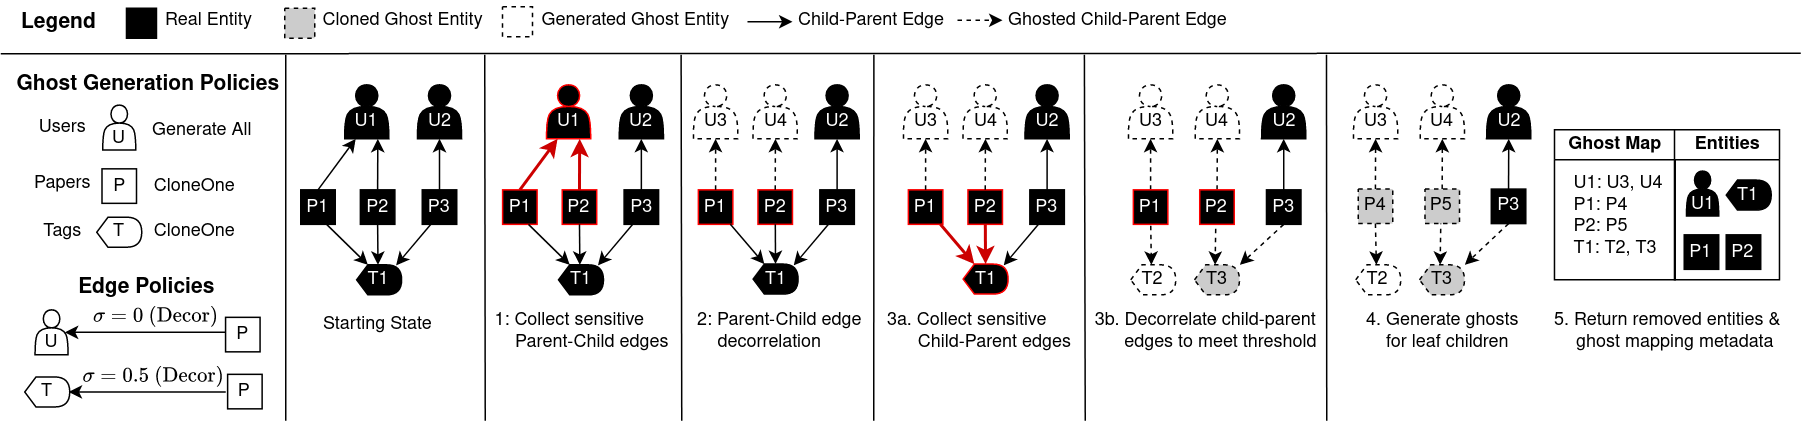
\includegraphics[width=\textwidth]{img/algo}

    \caption{Stages of \sys's execution when unsubscribing user U1. Entities and edges detected as
    sensitive are outlined in red. Only the part of the entity graph relevant to unsubscription is shown.
    For simplicity, the specified ghosting policies apply for all attributes
    of the entity: a black ghost entity indicates that it is a full clone of the original.
    New edges indicates that the edge (foreign-key) value of the child has been changed to
    point to the specified parent.\\
    In this example, \sys decorrelates paper-tag edges only enough that the proportion of sensitive papers
    is at most the sensitivity threshold of 0.5, retaining one correlation between a sensitive
    paper P2 and the parent tag T1, and decorrelating the other sensitive paper P1 from the tag.}
    \label{fig:algo}
\end{figure*}


Given an application's schema and unsubscription policy, and an entity to be decorrelated as input,
\sys executes unsubscription as follows. Figure~\ref{fig:algo} illustrates each step.
\begin{enumerate}
    \item \textbf{Parent-Child Traversal:} \sys traverses the entity graph starting from the input entity,
        going down parent to child edges (and halting if it detects a cycle). 
        \sys collects traversed edges as it traverses the graph. 
    
    \item \textbf{Parent-Child Edge Policy Application:} 
        Post-traversal, \sys acts on each collected edge instance according to the specified
        decorrelation relationship policy for that edge's type.

        \sys takes all edges of every unique parent entity, and applies policies as appropriate.
        Note that any sensitivity threshold less than $1$ requires that \emph{all} edges be decorrelated or
        deleted, depending on the developer's specified choice: all the children of this parent are
        sensitive due to the nature of \sys's parent-child traversal.

        Any edges that should be deleted removes the child entity and any descendants.
        \sys generates new ghost parents using the real parent as template for any edges that should
        be decorrelated, and rewrites the child's edge attribute to be the ghost parent's
        identifier. If any edges are retained, \sys generates a ghost parent entity to replace the
        parent.
      
    \item \textbf{Child-Parent Edge Policy Application:} 
        Next, \sys takes the children of all traversed edge instances, and considers the set of
        edges from these children to other parents \emph{not} traversed by \sys during the first
        traversal phase. In other words, these children have multiple parents, at least one of which
        is transitively connected to the input entity.

        Intuitively, children of edges traversed by \sys share a connection with the initial
        entity being decorrelated. Edges \emph{from} these children to other parent entities may
        thus leak sensitive identifying information. 

        \sys acts on these child-parent edges according to the specified edge policy for each edge's
        type. For each unique parent, \sys limits the proportion of edges of each type that connect
        to sensitive entities (the children of traversed edge instances) to below the policy's
        sensitivity threshold by either decorrelating or deleting the children. 
        If \sys retains any edges from sensitive children to the real parent, then \sys generates a
        ghost parent entity to replace the parent.
        
        Note that unlike the previous steps, this step considers edges from parents that may have
        many non-sensitive children (\eg a particular tag may correlate with many stories by various
        authors).  \sys therefore may retain edges to sensitive children when given a sensitivity
        threshold less than 1 and greater than 0, unlike in the previous step.

        \sys optionally allows developers to specify that edges have weaker or stronger edge
        policies in the child-to-parent direction than in the  parent-to-child direction. Weaker
        policies---higher sensitivity thresholds---allow \sys to retain links if \emph{only the
        child} is sensitive, but decorrelate or remove the link if \emph{both} the child and parent
        are sensitive. For example, perhaps a user wants to ensure that they are decorrelated from
        their reviews, but correlations between the review and the the paper authors can still be
        retained.

        Stronger policies may specify that the parent connected to sensitive children should
        decorrelate \emph{all} correlations to the paper even from non-sensitive correlations.
        Developers specify such a policy with a sensitive threshold of -1. For
        example, perhaps the set of users with review conflicts to the paper can identify the
        author, even if the author is decorrelated from the paper. We see an example of this in
        Section~\ref{sec:hotcrp_example} (Figure~\ref{fig:pcs}).

    \item \textbf{Anonymizing Leaf Children:}
        If any sensitive children that are leaves (have no children) remain, \sys generates a ghost child entity to replace this leaf.
        
        In Figure~\ref{fig:algo}, step 4, P1 and P2 are both leaves. \sys generates ghosts for both
        these papers: since these papers have \texttt{CloneOne} ghosting policies, ghost papers gP1
        and gP2 are identical to P1 and P2, and retain the edge attributes linking them to their
        respective parent tags and users.

    \item \textbf{Returning User Data:} \sys collects all removed entities that have either been
        replaced by ghost entities, or deleted entirely from the graph. \sys also records all
        generated ghost entity identifiers, and which ghost entities replaced which real entity.
        \sys returns both the removed entity data and this ghost entity metadata to the user.
\end{enumerate}

Note that \sys must decide \emph{which} ghost clones the template entity's attributes when the
developer selects a \texttt{CloneOne} ghosting policy for one or more attributes. \sys always
associates the cloned ghost with as many non-sensitive entities as possible. For example, as shown
in Figure~\ref{fig:algo} step 3b, if \sys decorrelates sensitive papers from a parent tag with a
\texttt{CloneOne} policy, \sys chooses the ghost tag that remains associated with non-sensitive
papers to be the clone. This decision ensures that any subscribed users and unsensitive application
data remain as unaffected as possible by another user's unsubscription. To optimize
\texttt{CloneOne} policies, \sys can simply retain the original template entity instead of producing
a cloned ghost.

\subsection{HotCRP's Unsubscription Policy}
\label{sec:hotcrp_example}
\begin{figure*}[t!]
    \centering
    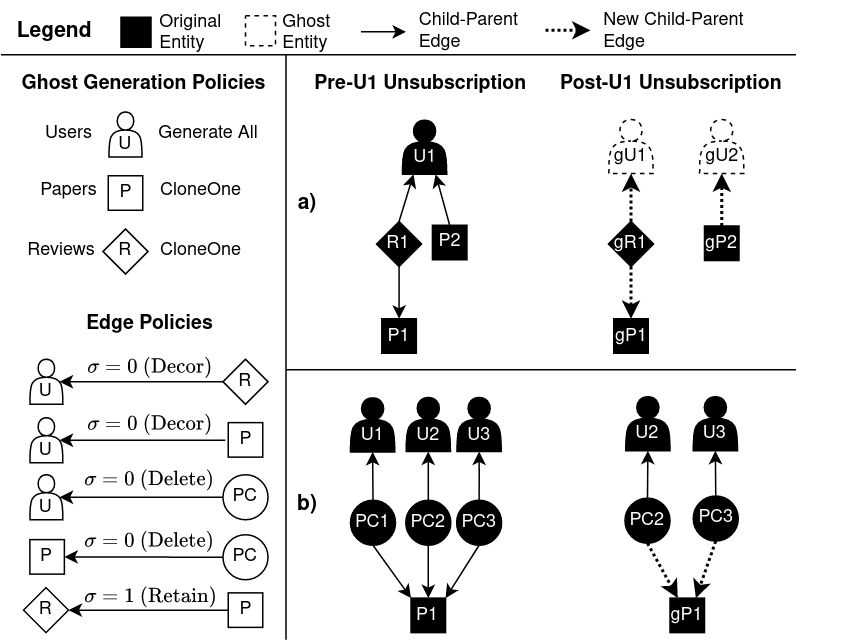
\includegraphics[width=\textwidth]{img/decor_hotcrp}

    \caption{Pre- and post-unsubscription state of user, paper, review, paper conflict, and paper
    tag entities based on a simplified variant of the HotCRP schema. \\ 
    \textbf{(a)} \sys decorrelates user-review and user-paper edges, and retains
    review-paper edges, generating ghost users randomly, but cloning each review and paper. \\
    \textbf{(b)} \sys decorrelates user-conflict edges and sensitive conflict-paper edges. The ghost
    paper associated with non-sensitive conflicts is a clone of the original; \sys generates a
    default placeholder paper as the ghost paper parent for the sensitive conflict.
    }
    \label{fig:hotcrp}
\end{figure*}

\begin{figure*}[ht!]
    \centering
    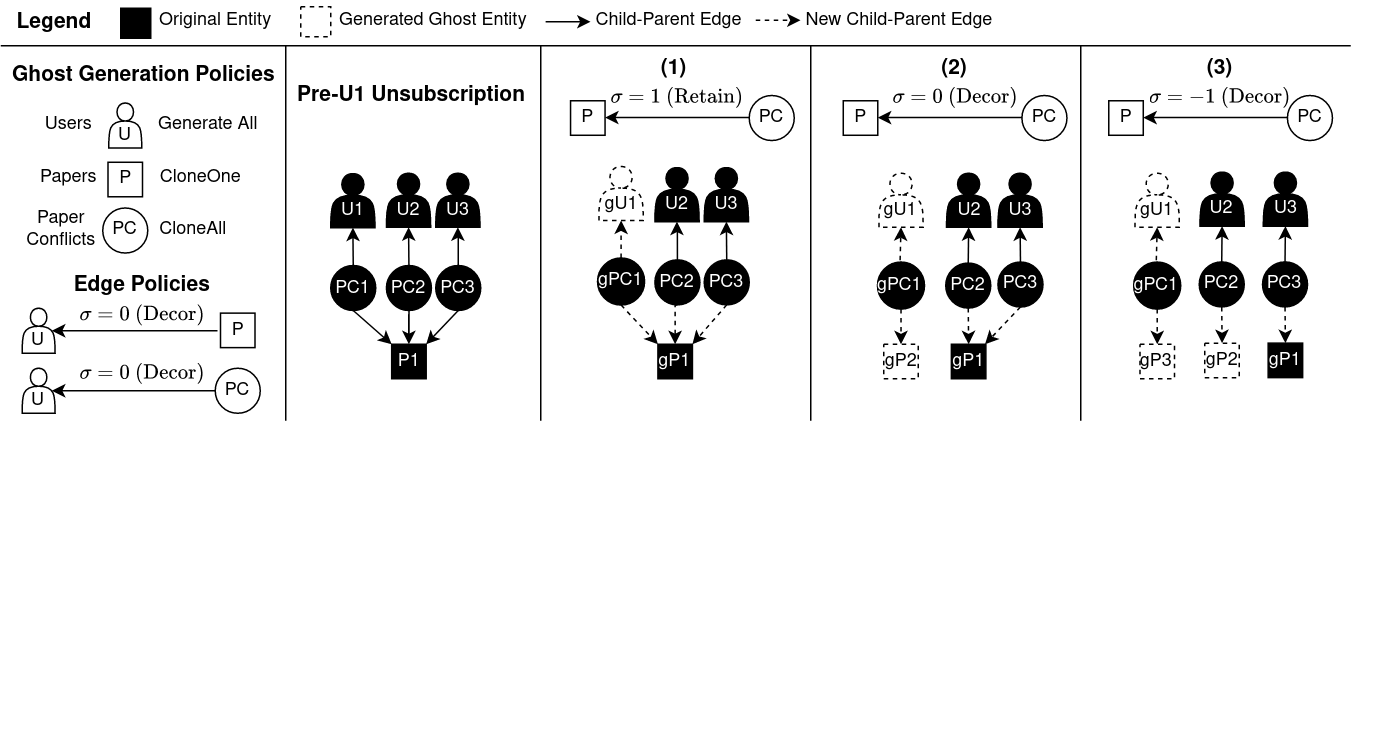
\includegraphics[width=\textwidth]{img/pcs}

    \caption{Different potential edge policies for paper-conflict to paper edges in HotCRP.
    (1) retains edges from sensitive paper conflicts to papers; (2) decorrelates sensitive
    paper conflicts from papers; (3) decorrelates all paper conflicts from papers.}
    \label{fig:pcs}
\end{figure*}

We next show how a developer would use \sys's design to write an unsubscription policy for HotCRP. 
HotCRP entities include users (reviewers and paper authors), papers, paper reviews, and paper
conflicts. There are a total of 25 entities, with 48 edge types between entities.
We illustrate how unsubscription changes a simplified HotCRP entity graph with users, papers,
reviews, paper conflicts, and tags in Figure~\ref{fig:hotcrp}.

The developer first specifies that the top-level entity to decorrelate is a user (entities of the
\texttt{ContactInfo} table). Users include authors and reviewers who may want to remove their
connections with their reviews, papers, and other metadata (such as papers they have requested to
review).

\paragraph{Generation Ghost Entities.}
Next, the developer should decide how \sys generates ghost for all entities. 
For simplicity, Figure~\ref{fig:hotcrp} shows entity-granularity ghosting policies
rather than per-attribute ghosting policies, and does not display the generation method (\eg random, default, etc.).

Most ghost user attributes should be assigned \texttt{GenerateAll} ghosting policies because no
profile information about the unsubscribing user should be retained. The developer may choose to
clone attributes such as the user's roles once, to ensure that the number of users with a certain
role does not change; however, any cloned attributes should not reveal any identifying information.
Finally, the developer should ensure that HotCRP never assigns ghost users papers to review: the
\texttt{disabled} attribute should be generated with a default value \texttt{true} for all ghosts.

In order to usefully retain paper and review information when a user unsubscribes, the developer chooses to
entirely clone all paper attributes in one ghost, and generate the other ghost papers with default
values for all attributes. Table~\ref{tab:ghosting} shows the partial specification for generation
ghost papers. Cloning the paper or review once to retain its information is safe: the developer knows that
paper attributes do not reveal identifying information.

In particular, it is safe to clone edges to user parents because the developer knows that \sys will decorrelate
edges to sensitive parents (replacing them with edges to ghost parents) \emph{prior} to ghosting the child
entity (the paper). Thus, any cloned edge attributes will necessarily point to ghosts if
there was a sensitive correlation between the paper and user parent.
We see a concrete example of this in Figure~\ref{fig:algo}: step 3b ensures that the
user and tag parents or any sensitive papers are appropriately ghosted prior to step 4, which ghosts
the paper.

Finally, the developer chooses to clone all paper conflicts. Paper conflicts have three attributes: one
specifies the conflict type (author or reviewer conflict), and the other two are edge attributes
that specify a user and a paper parent. It is safe to clone conflict types because this reveals
little identifying information, and does not interfere with HotCRP's execution. As with paper
entities, it is safe to clone edges to user and paper parents because any cloned edge attributes
will necessarily point to ghosts if there was a sensitive correlation between paper conflicts and parent entity.

\paragraph{Specifying Edge Policies.}
All direct correlations between a user and the user's reviews, papers, paper conflicts, and other
data may leak the user's identity. The developers therefore specifies edge policies with a
sensitivity threshold of 0 for edges of with the user as a direct parent.  Because HotCRP should
retain the paper and review data, and merely decorrelate these data from their author's identity,
the developer specifies that \sys should decorrelate these edges to meet the threshold: \sys will
replace any edges from papers or reviews to the unsubscribing user with an edge to a ghost user
profile. Figure~\ref{fig:hotcrp}a shows how \sys decorrelates a user from
their reviews and papers.

Although parent-child links from users to their data should be decorrelated during unsubscription,
HotCRP should maintain correlations between other subscribed users and sensitive papers, reviews,
and other entities. Thus, the developer specifies a weaker edge policy in the child-parent
direction (papers-to-users, reviews-to-users, etc.) with sensitivity threshold 1, allowing these
correlations to remain unchanged.

As observed earlier, edges that are not directly linked to the user may also reveal identifying
information about the user's identity: the group of collaborators or conflicting members of the PC
may pinpoint the identity of the ``ghost user'' on a paper. Users are linked to papers via
\emph{paper conflict} entities, which have both a user and a paper as a parent.  Paper conflicts can
either indicate authorship or a reviewer conflict (prior collaborators or sharing an institution).
When a user unsubscribes, the edge policies described above ensure that the user is decorrelated from
their paper conflicts. However, the developer must also ensure that edges from these sensitive paper
conflicts their parent papers cannot leak identifying information.

Here, the developer can make one of three choices. These choices demonstrate the tradeoff between
retaining information for application correctness, and completely de-identifying the user.
Figure~\ref{fig:pcs} shows how each choice choices affects the post-unsubscription application state.
%
The first choice leaves correlations between sensitive paper conflicts and papers in place.
This allows other users to see that some ghost user has a conflict with the paper, and potentially
derive the user's identity by deducing the users' affiliation or collaborators based on the
paper conflicts between the paper and other users.

The second choice decorrelates sensitive paper conflicts from the paper with a sensitivity threshold
of 0. This ensures that each sensitive paper conflict will be associated with a ghost paper parent
after unsubscription. To other users who can view the paper, it will appear as the sensitive paper
conflict never existed. Unlike the first choice, this can lead to spurious, unexplained conflicts:
for example, the PC may observe that a reviewer who works at BU has a conflict with a paper, but
none of the paper's authors are from BU (because the author unsubscribed, and their conflict was
decorrelated from the paper). Spurious conflicts can lead to identifying information leakage: in
this case, observers can see at least one unsubscribed user likely works at BU. However, unlike the
first choice, other users cannot be sure of exactly how many unsubscribed users and conflicts
initially existed, and if no spurious conflicts are produced, cannot deduce that an unsubscribed
user had a conflict at all. In addition, if the unsubscribed user had a reviewer conflict instead of
a author conflict with the paper, then this choice leaks no identifying information at all.

The third choice decorrelates \emph{all} paper conflicts correlations with the paper. While this
certainly removes all potentially identifying information derivable from paper conflicts, this
breaks HotCRP semantics: users who should not be able to view the paper (due to conflicts) will
suddenly be able to.
\lyt{TODO: right now, only sensitive children can be decorrelated in the child-parent direction}

To balance between maintaining application correctness and de-identifying the user, we choose the
second edge policy for paper-conflict to paper edges, shown in Figure~\ref{fig:hotcrp}b.
If the user resubscribes, the decorrelated paper conflict is relinked to the user and the original
paper, restoring the original state.  If all users with conflicts to the same paper decorrelate, the
paper will have no associated user accounts.

%The HotCRP developer may also determine that tags can identify a user if only that user's papers are
%associated with that tag. The developer thus specifies that paper-tag edges have a sensitivity
%threshold of 0.5: at most half the papers with that tag can be associated with the unsubscribing
%user. \sys decorrelates these edges until the threshold is met; all ghost tag attributes are
%generated using a clone-one ghosting policy.  Figure~\ref{fig:hotcrp}c shows how \sys partially
%decorrelates a user's papers from a shared tag parent.
%\lyt{I know this doesn't exactly reflect HotCRP's schema (which uses PaperTags to link papers to
%tags), but I found this example the most convincing to demonstrate partial decorrelation. This may
%be more relevant in a different application than HotCRP.}

The final group of edge policies ensure that review and paper artifacts remain present
and correctly linked with other application entities: (subscribed) reviewers should still see the
correct paper for each of their reviews, (subscribed) authors should see the correct reviews for
their papers, and review and paper metadata should remain correctly associated. The developer
specifies a sensitivity threshold of 1 for all edge types that were not assigned a policy in the
prior steps, indicating that \sys should leave these edges untouched.

%\sys provides a menu of unsubscription policy choices that allow developers to choose how to
%\emph{ghost} individual data record content, and how to \emph{decorrelate} sensitive correlations. 
%Specifying the policy requires nothing more than the application schema: ghosting policies act on
%application datatables and on foreign key relationships between tables.
%Table column values can be ghosted---removed, anonymized, or modified---in application-specific
%ways; and correlations can be broken, removed, or desensitized by adding noise. This gives
%developers the flexibility to specify fine-grained policies that properly de-identify a user, while
%retaining data as necessary for the application.

%\sys must pinpoint exactly which data and correlations may be
%identity-sensitive, and allow developers to specify exactly what the post-unsubscription state of
%this data should be.
